\documentclass[fleqn,10pt]{olplainarticle}
\usepackage{hyperref}

\usepackage{xcolor}
\hypersetup{
	colorlinks,
	linkcolor={red!50!black},
	citecolor={blue!50!black},
	urlcolor={blue!80!black}
}

\usepackage{enumitem}

\usepackage{float}

\usepackage{caption}
\usepackage{subcaption}
\usepackage{multicol}

\usepackage{lscape}
\usepackage{makecell}

\usepackage{color}
\usepackage{colortbl}

\usepackage{pgfplots}

\usepackage{xurl}
%%%%%%%%%%%%%%%%%%%%%%%%%%%%%%%%%%

%%solidity code%%%%%%%%%%%%%%%%%%%
% Copyright 2017 Sergei Tikhomirov, MIT License
% https://github.com/s-tikhomirov/solidity-latex-highlighting/

\usepackage{listings, xcolor}

\definecolor{verylightgray}{rgb}{.97,.97,.97}

\lstdefinelanguage{Solidity}{
	keywords=[1]{anonymous, assembly, assert, balance, break, call, callcode, case, catch, class, constant, continue, constructor, contract, debugger, default, delegatecall, delete, do, else, emit, event, experimental, export, external, false, finally, for, function, gas, if, implements, import, in, indexed, instanceof, interface, internal, is, length, library, log0, log1, log2, log3, log4, memory, modifier, new, payable, pragma, private, protected, public, pure, push, require, return, returns, revert, selfdestruct, send, solidity, storage, struct, suicide, super, switch, then, this, throw, transfer, true, try, typeof, using, value, view, while, with, addmod, ecrecover, keccak256, mulmod, ripemd160, sha256, sha3}, % generic keywords including crypto operations
	keywordstyle=[1]\color{blue}\bfseries,
	keywords=[2]{address, bool, byte, bytes, bytes1, bytes2, bytes3, bytes4, bytes5, bytes6, bytes7, bytes8, bytes9, bytes10, bytes11, bytes12, bytes13, bytes14, bytes15, bytes16, bytes17, bytes18, bytes19, bytes20, bytes21, bytes22, bytes23, bytes24, bytes25, bytes26, bytes27, bytes28, bytes29, bytes30, bytes31, bytes32, enum, int, int8, int16, int24, int32, int40, int48, int56, int64, int72, int80, int88, int96, int104, int112, int120, int128, int136, int144, int152, int160, int168, int176, int184, int192, int200, int208, int216, int224, int232, int240, int248, int256, mapping, string, uint, uint8, uint16, uint24, uint32, uint40, uint48, uint56, uint64, uint72, uint80, uint88, uint96, uint104, uint112, uint120, uint128, uint136, uint144, uint152, uint160, uint168, uint176, uint184, uint192, uint200, uint208, uint216, uint224, uint232, uint240, uint248, uint256, var, void, ether, finney, szabo, wei, days, hours, minutes, seconds, weeks, years},	% types; money and time units
	keywordstyle=[2]\color{teal}\bfseries,
	keywords=[3]{block, blockhash, coinbase, difficulty, gaslimit, number, timestamp, msg, data, gas, sender, sig, value, now, tx, gasprice, origin},	% environment variables
	keywordstyle=[3]\color{violet}\bfseries,
	identifierstyle=\color{black},
	sensitive=true,
	comment=[l]{//},
	morecomment=[s]{/*}{*/},
	commentstyle=\color{gray}\ttfamily,
	stringstyle=\color{red}\ttfamily,
	morestring=[b]',
	morestring=[b]"
}

\lstset{
	language=Solidity,
	backgroundcolor=\color{verylightgray},
	extendedchars=true,
	basicstyle=\footnotesize\ttfamily,
	showstringspaces=false,
	showspaces=false,
	numbers=left,
	numberstyle=\footnotesize,
	numbersep=9pt,
	tabsize=2,
	breaklines=true,
	showtabs=false,
	captionpos=b
}


%%%%%%%%%%%%%%%%%%%%%%%%%%%%%%%%%%

%%Block color quote%%%%%%%%%%%%%%%

\usepackage[most]{tcolorbox}

\definecolor{linequote}{RGB}{224,215,188}
\definecolor{backquote}{RGB}{249,245,233}

\newtcolorbox{myquote}[1][]{%
	enhanced, breakable, 
	size=minimal,
	frame hidden, boxrule=0pt,
	sharp corners,
	colback=backquote,
	#1
}

%%%%%%%%%%%%%%%%%%%%%%%%%%%%%%%%%%

% Use option lineno for line numbers 

\title{Storage Strategies for Gas Reduction}

\author[1]{jistro.eth~~~~0xVato.stark}
%\author[2]{Ariutokintumi.eth }
%\affil[1]{Address of first author}
%\affil[2]{Address of second author}

\keywords{EVM, Blockchain}


\begin{abstract}
The objective of this research is to efficiently store any number of native or non-native tokens for an account while minimizing the gas consumption for each transaction. This goal is pursued without accounting for the deployment cost of the contract.
\end{abstract}

\begin{document}

\flushbottom
\maketitle
\thispagestyle{empty}

\tableofcontents

\section{First Iteration: Implementation of Mappings}
During this phase, a smart contract is implemented employing a specific strategy. The use of a \texttt{mapping} is more gas-efficient than implementing with dimensional or multi-dimensional arrays \cite{natewelch__answer_2018}. The implementation utilizes a \texttt{public} nested \texttt{mapping}, where the first key (\texttt{address}) represents the account, and the subsequent key (\texttt{address}) corresponds to the smart contract of the token. This structure allows us to retrieve the holdings for a specific account in this token, represented by \texttt{uint256}.
\begin{myquote}[colback=gray!30, size=small]
It's crucial to note that, for each smart contract implemented, the compiler version used is 0.8.20, utilizing the Shanghai EVM version. All tests are conducted using an account with 10,000 registered addresses. This choice is based on the observation of a linear pattern in gas consumption when testing with 100, 1000, and 10,000 mock token addresses. As there were no drastic changes in the pattern, we have chosen to keep the number of registered addresses at 10,000 for consistency.
\end{myquote}
Based on the code from \url{https://github.com/Roll-a-Mate/Research/blob/main/0004-Storage%20Strategies%20for%20Gas%20Reduction/code/src/FirstApproach.sol}, using the \texttt{entryInit}, \texttt{entryAdd}, and \texttt{entrySub} functions, the gas consumption results are shown in Table \ref{tab:FirstIT}.

\begin{table}[H]
	\centering
	\begin{tabular}{|l|l|l|l|l|}
		\hline
		Name       & min    & avg   & median &  max   \\ \hline
		entryInit  & 22752  & 22752 & 22752  &  22752 \\ \hline
		entryAdd   & 945  	& 945 	& 945  	 &  945   \\ \hline
		entrySub   & 923  	& 923 	& 923    &  923   \\ \hline
		mean       &\cellcolor{black}&\cellcolor{black}&\cellcolor{black}&8207\\ \hline
	\end{tabular}
	\caption{Gas Consumption Results for the First Iteration}
	\label{tab:FirstIT}
\end{table}


This serves as the foundation for subsequent iterations in the implementation of new strategies, eliminating the need for comparisons.

\section{Second Iteration: Implementation of Modifiers}

In this iteration, we introduce different modifiers to optimize transaction costs. For example, minimizing the use of \texttt{public} variables can significantly reduce gas expenses. \texttt{Public} variables implicitly generate a getter function, contributing to increased contract size and gas usage. To enhance efficiency, functions should be marked as \texttt{external} whenever possible. \texttt{External} functions are more gas-efficient than public ones, as they expect arguments to be passed from the external call, ultimately saving gas \cite{malanii_solidity_2023}. \\
Based on the code from \url{https://github.com/Roll-a-Mate/Research/blob/main/0004-Storage%20Strategies%20for%20Gas%20Reduction/code/src/SecondApproach.sol}, using the \texttt{private} keyword for variables and \texttt{external} for functions, the gas consumption results are shown in Table \ref{tab:SecondIT}.

\begin{table}[H]
	\centering
	\begin{tabular}{|l|l|l|l|l|}
		\hline
		Name       & min    & avg   & median &  max   \\ \hline
		entryInit  & 22730  & 22730 & 22730  &  22730 \\ \hline
		entryAdd   & 923  	& 923 	& 923  	 &  923   \\ \hline
		entrySub   & 901  	& 901 	& 901    &  901   \\ \hline
		mean       &\cellcolor{black}&\cellcolor{black}&\cellcolor{black}&8185\\ \hline
	\end{tabular}
	\caption{Gas Consumption Results for the Second Iteration}
	\label{tab:SecondIT}
\end{table}

Based on the mean total cost of the transaction, a change of -0.27\% (22 gas) is observed.

\section{Third Iteration: Reduction of Nested Mappings}

In this iteration, we aim to reduce the cost associated with using nested mappings by implementing a theoretical reduction in nested storage. To achieve this, we introduce a \texttt{bytes32} key to retrieve the balance of a specific token. This is accomplished by hashing the \texttt{address} of the account with the \texttt{address} of the token, the use of \texttt{bytes32} as the key is because this type of variables is the most optimized storage type \cite{malanii_solidity_2023,riady_how_2021}.\\
Based on the code from
\url{https://github.com/Roll-a-Mate/Research/blob/main/0004-Storage%20Strategies%20for%20Gas%20Reduction/code/src/ThirdApproach.sol}, using the \texttt{sha256} keyword for hashing, the gas consumption results are shown in Table \ref{tab:ThirdIT}.

\begin{table}[H]
	\centering
	\begin{tabular}{|l|l|l|l|l|}
		\hline
		Name       & min    & avg   & median &  max   \\ \hline
		entryInit  & 23455  & 23455 & 23455  &  23455 \\ \hline
		entryAdd   & 1621  	& 1621 	& 1621   &  1621   \\ \hline
		entrySub   & 1599  	& 1599 	& 1599   &  1599   \\ \hline
		mean       &\cellcolor{black}&\cellcolor{black}&\cellcolor{black}&8891\\ \hline
	\end{tabular}
	\caption{Gas Consumption Results for the Third Iteration}
	\label{tab:ThirdIT}
\end{table}

Compared to the first iteration, this iteration shows a 8.33\% increase in gas consumption (684 gas units) in the mean total cost. This indicates a more expensive implementation, leading us to discard this approach.

\section{Fourth Iteration: Implementation of \texttt{payable} in Functions}

In this iteration, we explore the introduction of the \texttt{payable} modifier in every function, aiming to achieve a slight improvement in gas efficiency compared to non-payable ones. The advantage lies in the fact that the compiler doesn't need to check for the transfer of Ether in payable functions, contributing to potential gas savings \cite{malanii_solidity_2023}.
Based on the code from \url{https://github.com/Roll-a-Mate/Research/blob/main/0004-Storage%20Strategies%20for%20Gas%20Reduction/code/src/FourthApproach.sol}, the gas consumption results are shown in Table \ref{tab:FourthIT}.

\begin{table}[H]
	\centering
	\begin{tabular}{|l|l|l|l|l|}
		\hline
		Name       & min    & avg   & median &  max   \\ \hline
		entryInit  & 22706  & 22706 & 22706  &  22706 \\ \hline
		entryAdd   & 899  	& 899 	& 899    &  899   \\ \hline
		entrySub   & 877  	& 877 	& 877    &  877   \\ \hline
		mean       &\cellcolor{black}&\cellcolor{black}&\cellcolor{black}&8161\\ \hline
	\end{tabular}
	\caption{Gas Consumption Results for the Fourth Iteration}
	\label{tab:FourthIT}
\end{table}


Compared to the first iteration, this iteration shows a decrease of 0.56\% (46 gas units).

\subsection{Concerns about \texttt{payable} in Functions}

The application of the \texttt{payable} modifier in functions raises substantial security concerns. Enabling primary token transfers within a function introduces potential risks, particularly when the specific actions or possibilities within this transaction are not fully comprehended. A meticulous evaluation of the security implications is imperative before integrating the \texttt{payable} modifier into any function. In this section, we will explore the criticality of these concerns.

Upon consulting the Slither Detector wiki \cite{trail_of_bits_detector_nodate} and reviewing pertinent security articles \cite{noauthor_smart_2023,noauthor_recommendations_nodate}, along with security audit documents \cite{watchpug_h04_nodate,berndartmueller_m01_nodate,chin_use_nodate}, it becomes evident that issues associated with the \texttt{payable} modifier primarily revolve around the transfer of native tokens into the contract, such as reentrancy or replay attacks using loops, etc. Notably, there is no documented evidence regarding specific payload executions.



\section{Fifth Iteration: Implementation of Linked Lists}

In this iteration, we explore the use of linked lists to retrieve token data for each transaction, aiming to achieve more gas-efficient transactions.

Based on the code from SoliChain \cite{boudjemaa_elevate_2023}, we implement this approach in our code available at \url{https://github.com/Roll-a-Mate/Research/blob/main/0004-Storage%20Strategies%20for%20Gas%20Reduction/code/src/FifthApproach.sol}. The gas consumption results are shown in Table \ref{tab:FifthIT}.


\begin{table}[H]
	\centering
	\begin{tabular}{|l|l|l|l|l|}
		\hline
		Name       & min    & avg   & median &  max   \\ \hline
		entryInit  & 25369  & 45267 & 45269  &  45269 \\ \hline
		entryAdd   & 1045  	& 1045 	& 1045   &  1045   \\ \hline
		entrySub   & 1067  	& 1067 	& 1067   &  1067   \\ \hline
		mean       &\cellcolor{black}&\cellcolor{black}&\cellcolor{black}&15794\\ \hline
	\end{tabular}
	\caption{Gas Consumption Results for the Fifth Iteration}
	\label{tab:FifthIT}
\end{table}

Compared to the first iteration, this approach results in a 92.78\% increase in gas consumption (7587 gas units) in the mean total cost. This indicates a very expensive implementation, leading us to discard this approach.

\section{Conclusion}

The investigation into optimizing gas consumption for transactions on Ethereum or compatible EVM chains has led to several iterations of smart contract implementations. Each iteration introduced specific strategies, and the gas consumption results were analyzed. Here's a summary of the conclusions drawn from each iteration: \\

\textbf{First Iteration: Implementation of Mappings} \\
Utilizing a \texttt{mapping} for storage proves to be more gas-efficient than using dimensional or multi-dimensional arrays. \\
The use of a \texttt{public} nested \texttt{mapping} provides a foundation for subsequent iterations.

\textbf{Second Iteration: Implementation of Modifiers} \\
Introduction of different modifiers, such as marking variables as \texttt{private} and functions as \texttt{external}, results in a decrease in gas consumption (0.27\%).

\textbf{Third Iteration: Reduction of Nested Mappings} \\
Attempting to reduce the cost of nested mappings by introducing a \texttt{bytes32} key increases gas consumption by 8.33\%. This approach is deemed more expensive and is discarded. \\
\textbf{Fourth Iteration: Implementation of \texttt{payable} in Functions} \\
Introducing the \texttt{payable} modifier in every function results in a small decrease in gas consumption (0.56\%).

\textbf{Fifth Iteration: Implementation of Linked Lists}\\
Implementing linked lists to retrieve token data significantly increases gas consumption (92.78\%), rendering this approach too expensive and unsuitable for optimization.
Overall, while some strategies led to marginal improvements, others proved to be more expensive. The choice of gas optimization strategy should be carefully considered based on the specific requirements and trade-offs in the context of the smart contract application.

\begin{figure}[h]
	\centering
	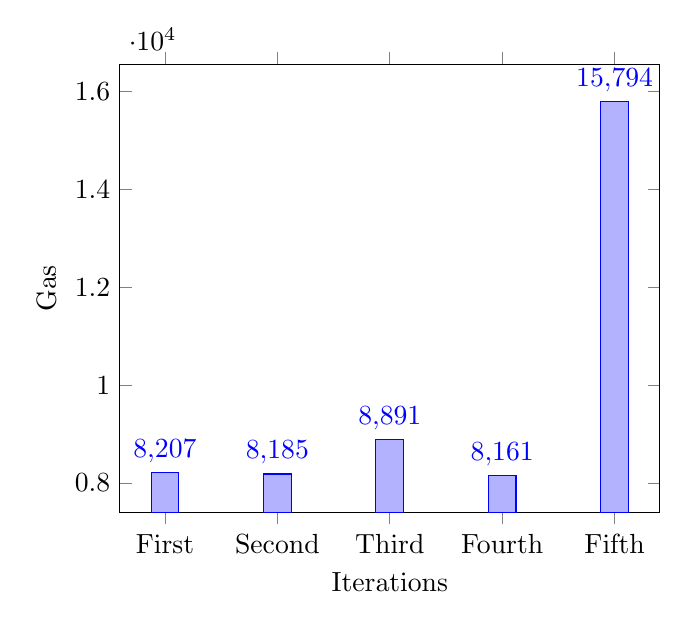
\begin{tikzpicture}
		\centering
		\begin{axis}[
			ybar,  
			ylabel=Gas,
			xlabel=Iterations,
			nodes near coords,
			symbolic x coords={First, Second, Third, Fourth, Fifth}, xtick=data,
			]
			\addplot 
			coordinates {(First,8207) (Second,8185) 
				(Third,8891) (Fourth,8161) (Fifth,15794)};
		\end{axis}
	\end{tikzpicture}
	\caption{Graph comparing Gas Consumption Results for each Iteration}
	\label{tab:Graph}
\end{figure}



\newpage
\bibliography{citations}

\end{document}